\maketitle
\tableofcontents

\vspace{0.5cm}


\section{Lösungsidee}\label{sec:losungsidee}
Das Problem der Aufgabenstellung beschreibt eine Variante des NP-vollständigen Traveling-Salesman Problems.
Es ist somit nicht möglich optimale Lösungen in polynomieller Zeit für beliebige Graphen zu finden.
Für die Graphen aus den Beispieldateien ist dies aufgrund ihrer Größe auch nicht möglich.
Folglich müssen zur Bewältigung der Aufgabe Heuristiken herangezogen werden. \\
Zunächst wird eine initiale Lösung mittels der Nearest-Neighbour Heuristik ermittelt.
Diese wird danach iterativ durch die TwoOpt-Postoptimierung verbessert.

\subsection{Nearest-Neighbour Heuristik}\label{subsec:nearest-neighbour-heuristik}
1.
Zunächst wird ein Startknoten \textit{v}\textsubscript{Start} ermittelt.
Ausgehend von \textit{v}\textsubscript{Start}, wird der Knoten \textit{v}\textsubscript{0} mit der geringsten Distanz gewählt.
\textit{v}\textsubscript{Start} und \textit{v}\textsubscript{0} werden als besucht markiert.
Die Kante \textit{e} zwischen diesen beiden Knoten wird für die Suche des nächsten Knotens genutzt.

2.
Solange es noch unbesuchte Knoten gibt, wird folgendes Verfahren wiederholt:
Betrachte in aufsteigender Distanz zu \textit{v}\textsubscript{0} alle Knoten.
Wenn die Kante, die den aktuell betrachteten Knoten und \textit{v}\textsubscript{0} verbindet \textit{e}
in einem stumpfen Winkel schneidet
Wähle unter allen nicht besuchten Knoten denjenigen Knoten \textit{v}, der die geringste Entfernung zu \textit{v}\textsubscript{0}
hat und gleichzeitig dessen Kante zu \textit{v}\textsubscript{0} \textit{e} in einem stumpfen Winkel schneidet (Winkelbedingung).

Ist es nicht möglich einen solchen Knoten zu finden, muss einen Schritt zurückgegangen werden und der

\subsection{TwoOpt Postoptimierung}\label{subsec:twoopt-postoptimierung}


\section{Umsetzung}\label{sec:umsetzung}
Die Implementierung erfolgt in Java 17.


\section{Beispiele}\label{sec:beispiele}
Die Beispiele entsprechen den Beispieldateien.
Beispiel 1 bis 3 lassen sich derart gut durch die Nearest-Neighbour Heuristik lösen, dass die Postoptimierung keine Verbesserungen erzielt.
Die Graphiken zeigen jeweils wie die ermittelte Tour verläuft und wie lang diese ist.
Gegebenenfalls sind zudem auch die Parameter der Postoptimierung angegeben.
Die vollständige Programmausgabe ist im Anhang zu finden.

\subsection{Beispiel 1}\label{subsec:beispiel-1}
\begin{figure}[h]
    \centering
    \begin{minipage}[b]{0.6\textwidth}
        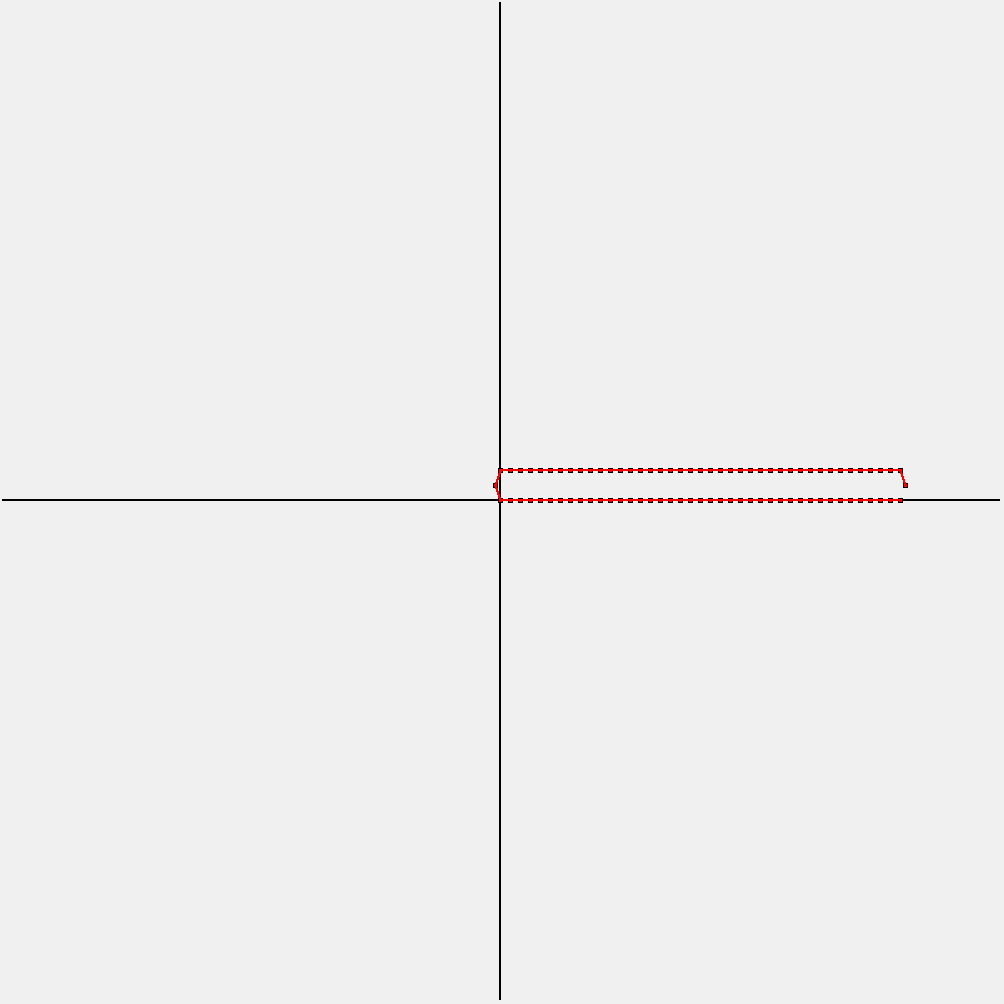
\includegraphics[width=\textwidth]{naivwenigerkrumm1}
        \caption{Naive Lösung Länge 847.4341649025257}
    \end{minipage}\label{fig:wenigerkrumm1}
\end{figure}
\FloatBarrier

\subsection{Beispiel 2}\label{subsec:beispiel-2}
\begin{figure}[h]
    \centering
    \begin{minipage}[b]{0.6\textwidth}
        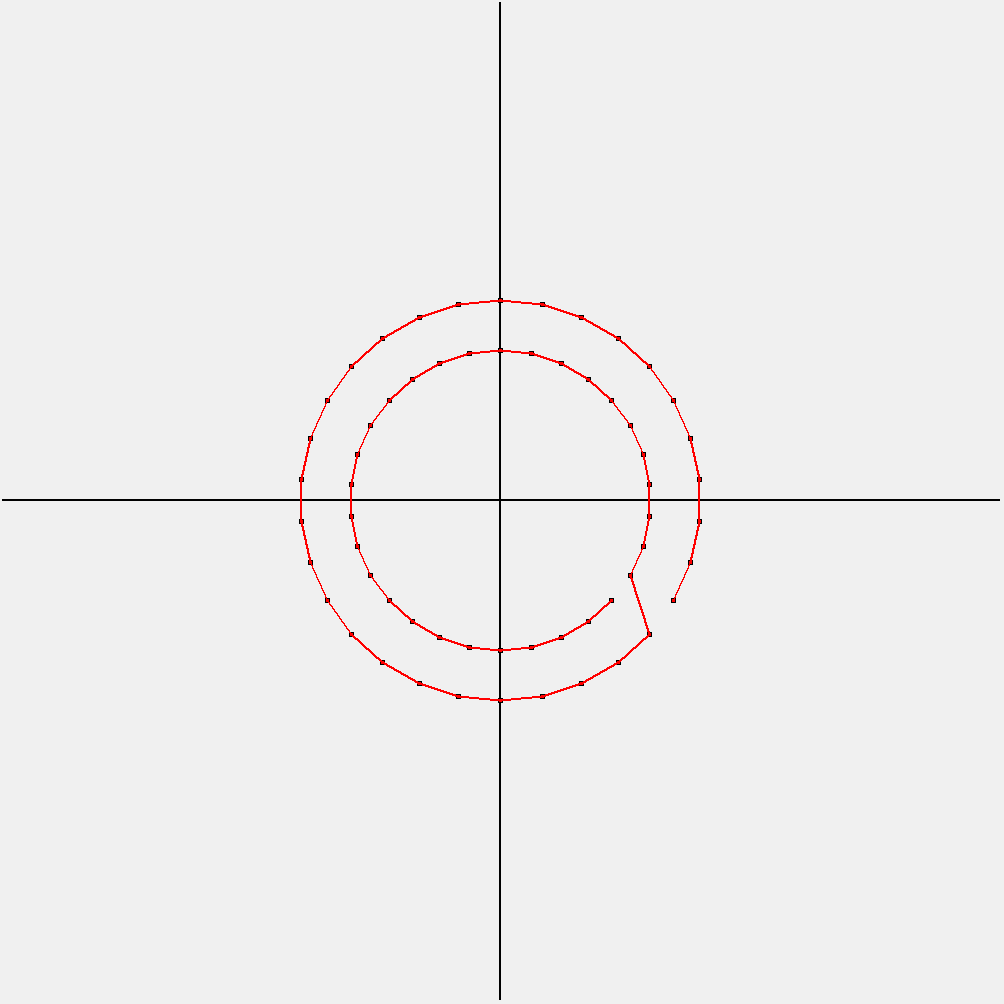
\includegraphics[width=\textwidth]{naivwenigerkrumm2}
        \caption{Naive Lösung Länge 2183.6622668054965}
    \end{minipage}\label{fig:wenigerkrumm2}
\end{figure}
\FloatBarrier

\subsection{Beispiel 3}\label{subsec:beispiel-3}
\begin{figure}[h]
    \centering
    \begin{minipage}[b]{0.6\textwidth}
        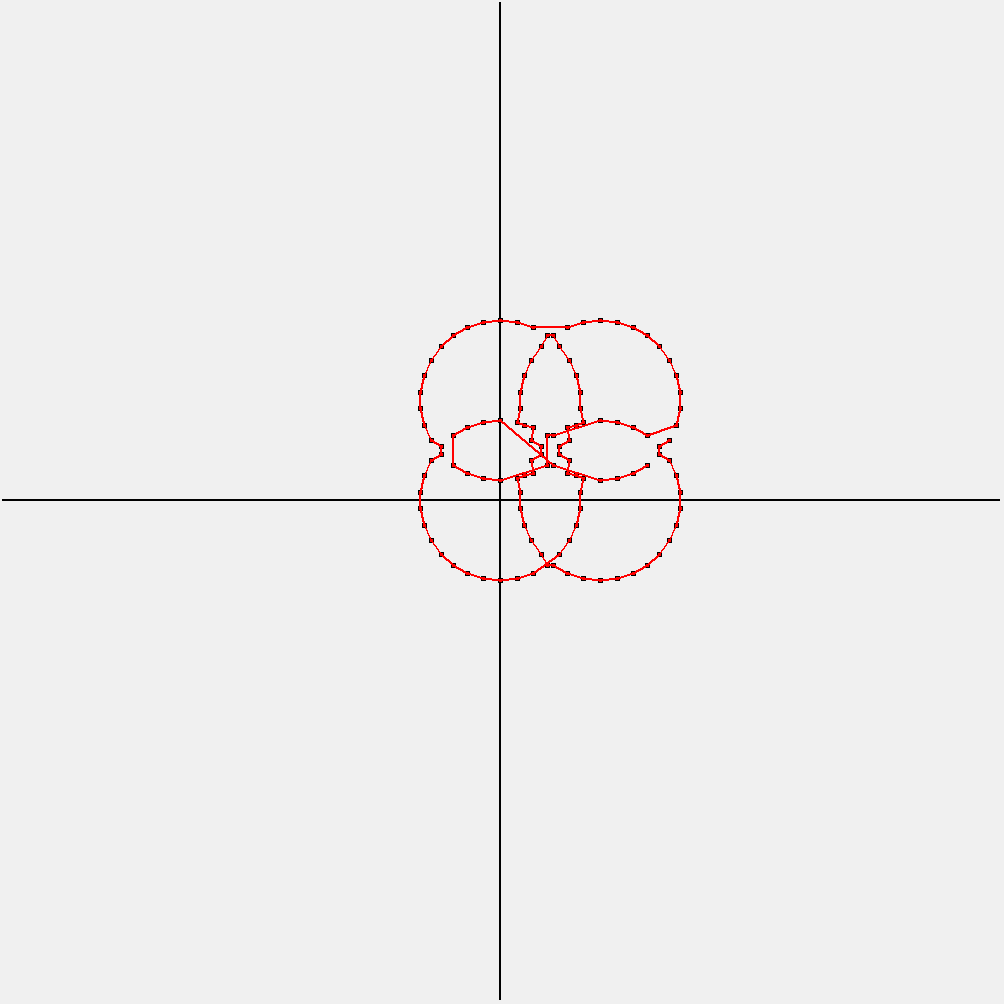
\includegraphics[width=\textwidth]{naivwenigerkrumm3}
        \caption{Naive Lösung Länge 2001.318764396512}
    \end{minipage}\label{fig:wenigerkrumm3}
\end{figure}
\FloatBarrier

\subsection{Beispiel 4}\label{subsec:beispiel-4}
\begin{figure}[h]
    \centering
    \begin{minipage}[b]{0.5\textwidth}
        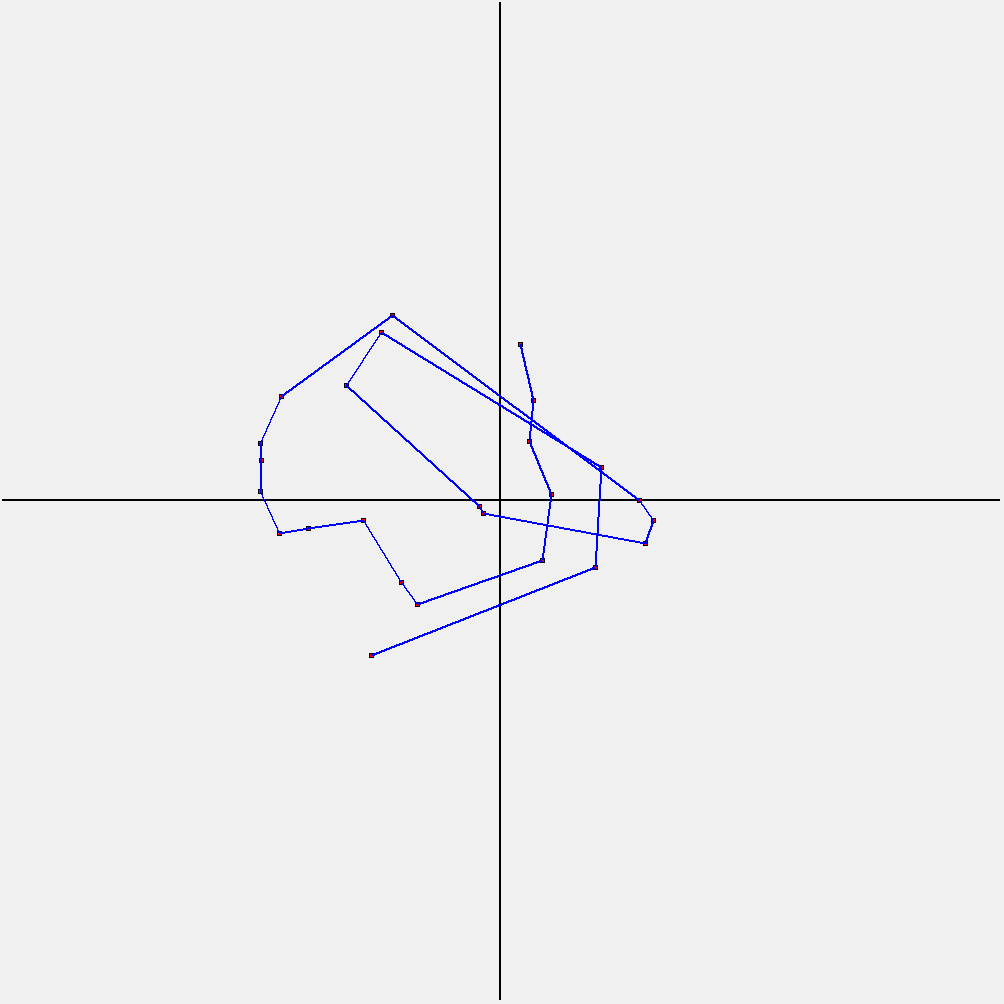
\includegraphics[width=\textwidth]{naivwenigerkrumm4}
        \caption{Naive Lösung Länge 2197.965650598992}
    \end{minipage}
    \hfill
    \begin{minipage}[b]{0.5\textwidth}
        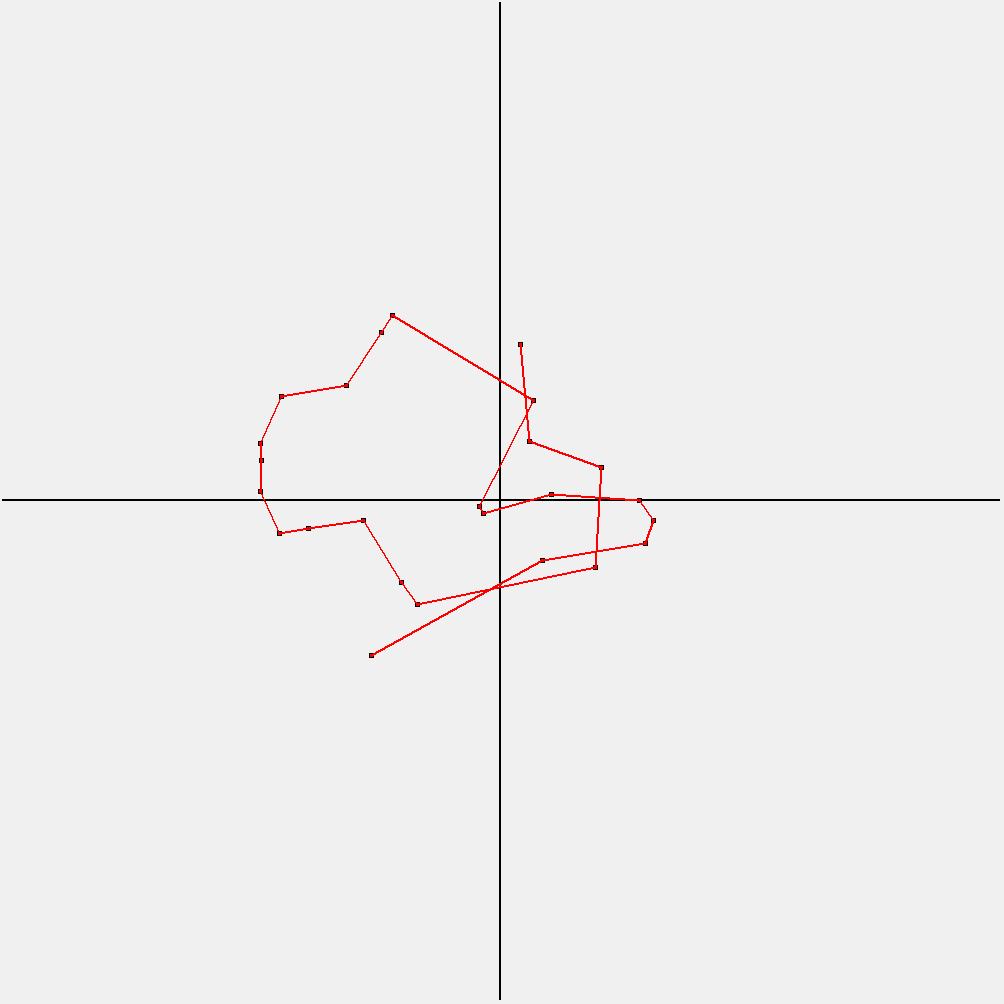
\includegraphics[width=\textwidth]{optimizedwenigerkrumm4}
        \caption{Optimierte Lösung Länge 1736.980701656645}
    \end{minipage}\label{fig:wenigerkrumm4}
\end{figure}
\begin{table}[b]
    \centering
    \begin{tabular}{|l|l|}
        \hline
        Parameter          & Wert  \\ \hline
        Starttemperatur    & 1300  \\ \hline
        Temperaturänderung & 0,985 \\ \hline
        \begin{tabular}[c]{@{}l@{}}
            Verbessernde Iterationen\\ bis zur Abkühlung
        \end{tabular}      & 10    \\ \hline
        \begin{tabular}[c]{@{}l@{}}
            Iterationen bis \\ zur Abkühlung
        \end{tabular}      & 16    \\ \hline
    \end{tabular}
    \caption{Parameterkonfiguration Beispiel 5}
    \label{tab:wenigerkrumm5}
\end{table}
\FloatBarrier

\subsection{Beispiel 5}\label{subsec:beispiel-5}
Zunächst wurde versucht mittels Nearest-Neighbour Heuristik eine initiale Lösung zu finden.
Dies führte auch nach über einer Stunde Laufzeit nicht zu einem Ergebnis.
Aufgrund dessen wurde die Nearest-Neighbour Heuristik derart modifiziert, dass nicht nur
der Abstand eines Knotens zum aktuellen Knoten in betracht gezogen wird, sondern auch
die Anzahl der möglichen Pfade die über den Knoten führen.
Je weniger solcher Pfade es gibt, desto höhere Priorität hat der Knoten in der Suche des nächsten Knotens.
Dieses Vorgehen erklärt die vergleichsweise schlechte initiale Lösung.
Um so interessanter ist es, dass die Postoptimierung dennoch zu so einem guten Ergebnis führt. \\

\begin{figure}[t]
    \centering
    \begin{minipage}[b]{0.5\textwidth}
        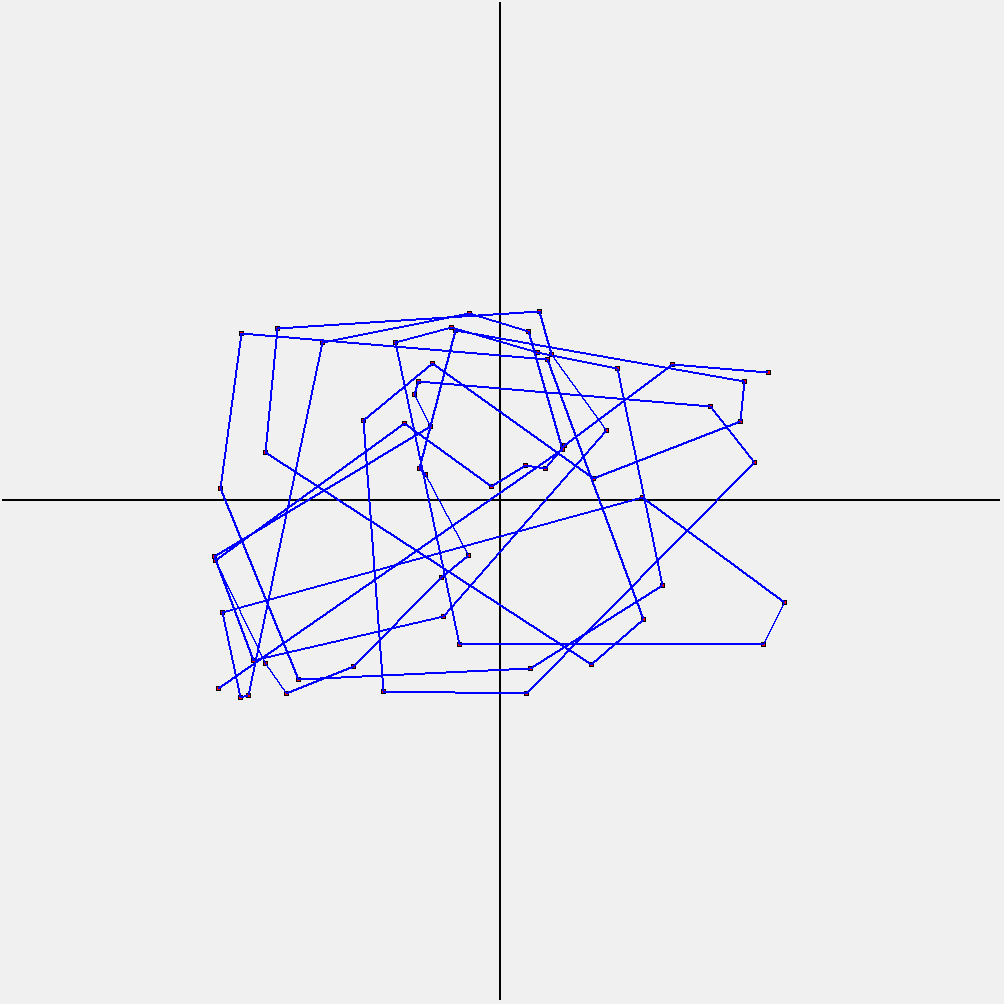
\includegraphics[width=\textwidth]{naivwenigerkrumm5}
        \caption{Naive Lösung Länge 9277.77985102936}
    \end{minipage}
    \hfill
    \begin{minipage}[b]{0.5\textwidth}
        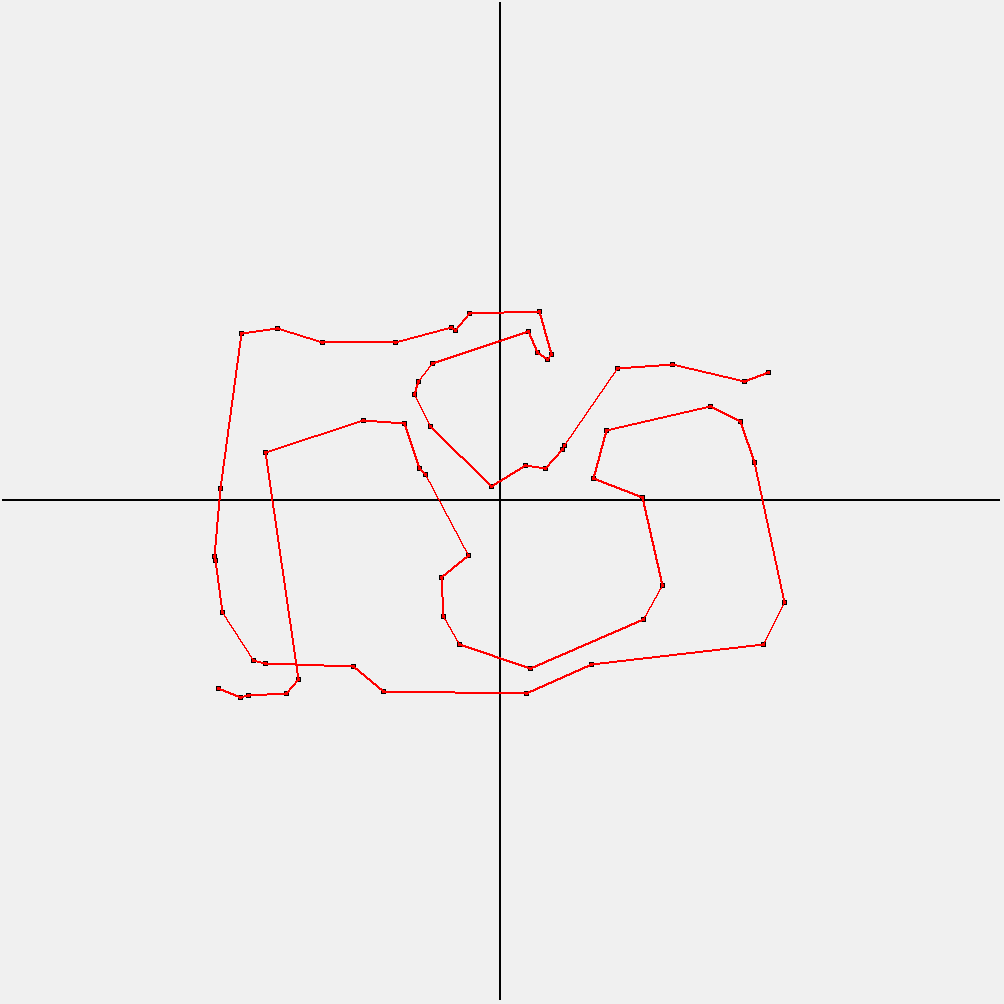
\includegraphics[width=\textwidth]{optimizedwenigerkrumm5}
        \caption{Optimierte Lösung Länge 3381.157719454162}
    \end{minipage}\label{fig:wenigerkrumm5}
\end{figure}

\begin{table}[b]
    \centering
    \begin{tabular}{|l|l|}
        \hline
        Parameter          & Wert  \\ \hline
        Starttemperatur    & 1300  \\ \hline
        Temperaturänderung & 0,985 \\ \hline
        \begin{tabular}[c]{@{}l@{}}
            Verbessernde Iterationen\\ bis zur Abkühlung
        \end{tabular}      & 10    \\ \hline
        \begin{tabular}[c]{@{}l@{}}
            Iterationen bis \\ zur Abkühlung
        \end{tabular}      & 16    \\ \hline
    \end{tabular}
    \caption{Parameterkonfiguration Beispiel 5}
    \label{tab:wenigerkrumm5}
\end{table}
\FloatBarrier
\subsection{Beispiel 6}\label{subsec:beispiel-6}

\begin{figure}[t]
    \centering
    \begin{minipage}[b]{0.6\textwidth}
        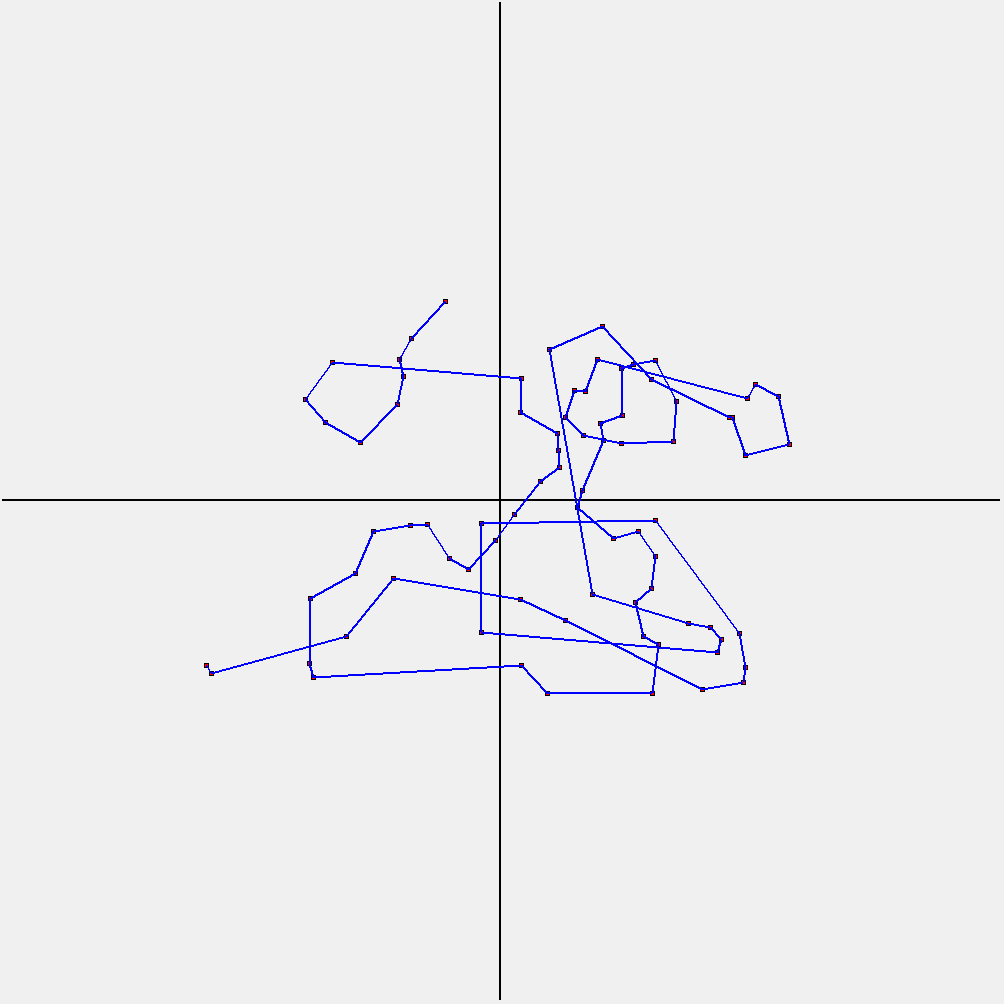
\includegraphics[width=\textwidth]{naivwenigerkrumm6}
        \caption{Naive Lösung Länge 4362.616434557695}
    \end{minipage}
    \hfill
    \begin{minipage}[b]{0.6\textwidth}
        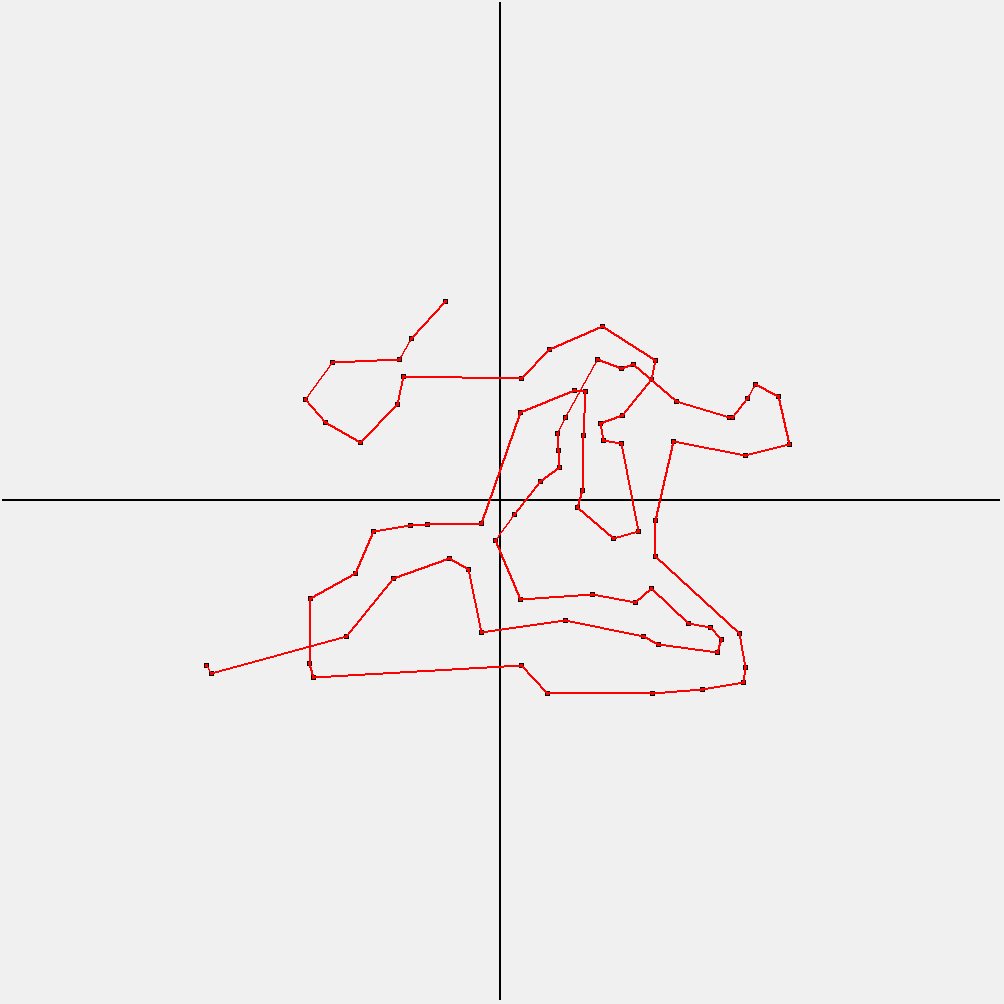
\includegraphics[width=\textwidth]{optimizedwenigerkrumm6}
        \caption{Optimierte Lösung Länge 3740.816749985773}
    \end{minipage}\label{fig:wenigerkrumm6}
\end{figure}

\begin{table}[b]
    \centering
    \begin{tabular}{|l|l|}
        \hline
        Parameter          & Wert  \\ \hline
        Starttemperatur    & 1300  \\ \hline
        Temperaturänderung & 0,985 \\ \hline
        \begin{tabular}[c]{@{}l@{}}
            Verbessernde Iterationen\\ bis zur Abkühlung
        \end{tabular}      & 10    \\ \hline
        \begin{tabular}[c]{@{}l@{}}
            Iterationen bis \\ zur Abkühlung
        \end{tabular}      & 16    \\ \hline
    \end{tabular}
    \caption{Parameterkonfiguration Beispiel 6}
    \label{tab:wenigerkrumm6}
\end{table}
\FloatBarrier

\subsection{Beispiel 7}\label{subsec:beispiel-7}

\begin{figure}[t]
    \centering
    \begin{minipage}[b]{0.5\textwidth}
        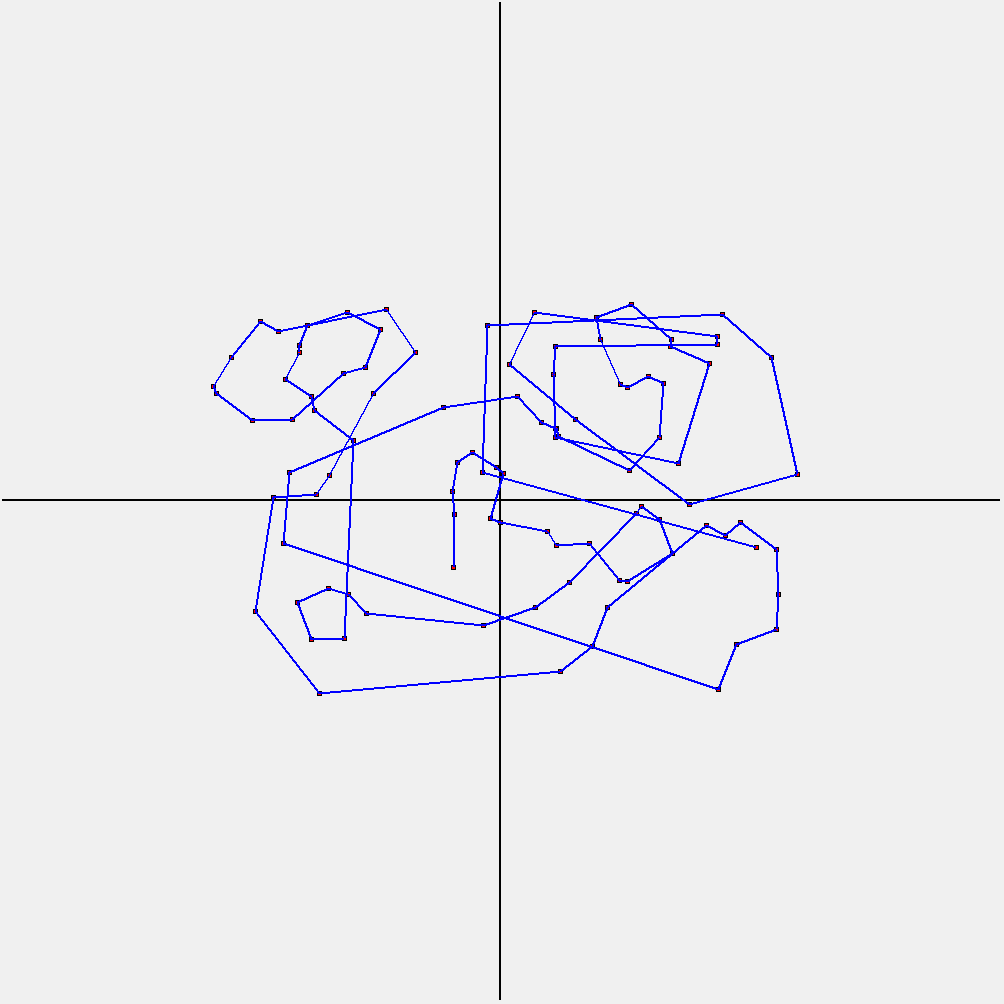
\includegraphics[width=\textwidth]{naivwenigerkrumm7}
        \caption{Naive Lösung Länge 6218.113121079488}
    \end{minipage}
    \hfill
    \begin{minipage}[b]{0.5\textwidth}
        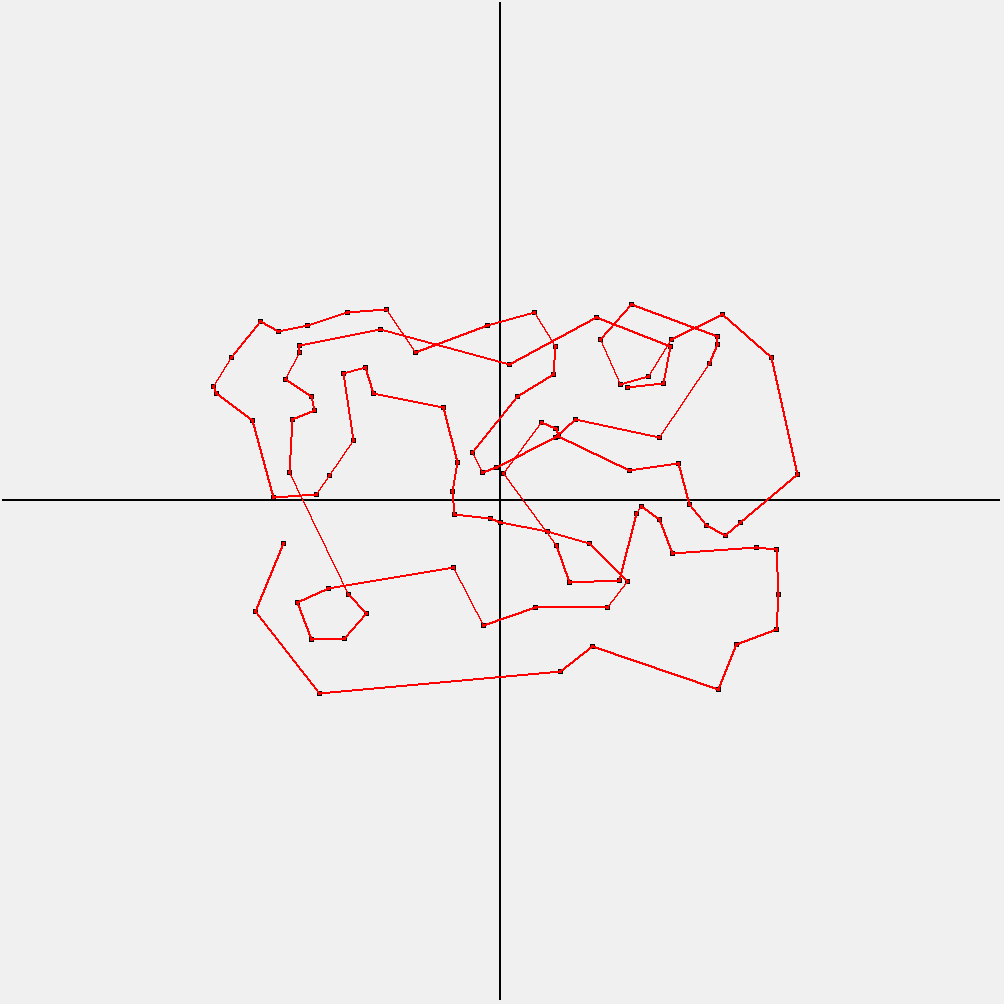
\includegraphics[width=\textwidth]{optimizedwenigerkrumm7}
        \caption{Optimierte Lösung Länge 4451.743885428826}
    \end{minipage}\label{fig:wenigerkrumm7}
\end{figure}

\begin{table}[b]
    \centering
    \begin{tabular}{|l|l|}
        \hline
        Parameter          & Wert  \\ \hline
        Starttemperatur    & 1450  \\ \hline
        Temperaturänderung & 0,975 \\ \hline
        \begin{tabular}[c]{@{}l@{}}
            Verbessernde Iterationen\\ bis zur Abkühlung
        \end{tabular}      & 10    \\ \hline
        \begin{tabular}[c]{@{}l@{}}
            Iterationen bis \\ zur Abkühlung
        \end{tabular}      & 19    \\ \hline
    \end{tabular}
    \caption{Parameterkonfiguration Beispiel 7}
    \label{tab:wenigerkrumm7}
\end{table}


\section{Quellcode}\label{sec:quellcode}
Unwichtige Teile des Programms sollen hier nicht abgedruckt werden.
Dieser Teil sollte nicht mehr als 2–3 Seiten umfassen, maximal 10.

